\chapter{Invariants}

De nombreux problèmes d'olympiades décrivent une situation que l'on transforme
en répétant une même opération. On demande alors si un certain état peut être
atteint, si le processus doit s'arrêter, ou quelle sera sa configuration finale.

Essayer toutes les suites d'opérations est souvent impossible. L'idée consiste
plutôt à chercher une propriété qui ne change jamais au cours du processus :
un \textbf{invariant}.

\section{Exemple introductif : retourner des jetons}

On dispose de \(8\) jetons, tous placés face blanche visible.

À chaque opération, on doit retourner exactement deux jetons.

Peut-on obtenir une configuration contenant exactement un jeton noir ?

\begin{center}
\fitfig{%
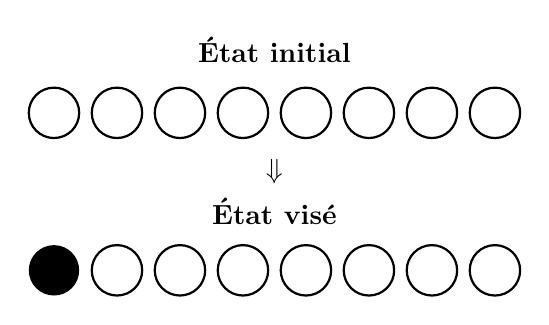
\begin{tikzpicture}[x=1cm,y=1cm,line width=0.8pt]
    \node at (3.5,2.8){\textbf{État initial}};
    \foreach \x in {0.7,1.5,2.3,3.1,3.9,4.7,5.5,6.3} \draw (\x,2) circle (0.32);
    \node at (3.5,1.25){\(\Downarrow\)};
    \node at (3.5,0.75){\textbf{État visé}};
    \fill (0.7,0) circle (0.32);
    \foreach \x in {1.5,2.3,3.1,3.9,4.7,5.5,6.3} \draw (\x,0) circle (0.32);
\end{tikzpicture}}
\end{center}

Notons \(N\) le nombre de jetons noirs.

Lorsqu'on retourne deux jetons, trois situations sont possibles :

\begin{itemize}
    \item deux jetons blancs deviennent noirs : \(N\) augmente de \(2\) ;
    \item un jeton blanc et un jeton noir sont retournés : \(N\) ne change pas ;
    \item deux jetons noirs deviennent blancs : \(N\) diminue de \(2\).
\end{itemize}

Ainsi, à chaque opération,

\[
N\longmapsto N+2,\qquad N,\qquad\text{ou}\qquad N-2.
\]

La parité de \(N\) ne change donc jamais.

Au départ,

\[
N=0,
\]

qui est pair. Après n'importe quel nombre d'opérations, \(N\) reste pair.

Or l'état demandé contient exactement un jeton noir, donc

\[
N=1,
\]

qui est impair.

L'état demandé est donc impossible à atteindre.

\[
\boxed{
\text{La parité du nombre de jetons noirs est un invariant.}
}
\]

\section{Le concept d'invariant}

\subsection{Définition}

Un \textbf{état} décrit complètement la situation à un instant donné.

Une \textbf{opération autorisée} transforme un état en un autre.

Une quantité \(I\) est appelée un \textbf{invariant} lorsqu'elle conserve
toujours la même valeur après chaque opération autorisée.

Autrement dit, si un état \(S\) est transformé en un état \(S'\), alors

\[
\boxed{I(S')=I(S).}
\]

On peut représenter le principe ainsi :

\begin{center}
\fitfig{%
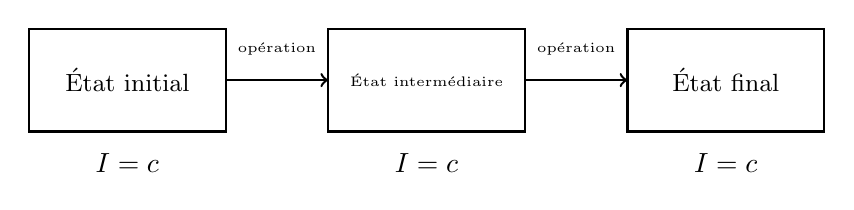
\begin{tikzpicture}[x=1cm,y=1cm,line width=0.9pt]
    \draw (0,0.5) rectangle (2.5,1.8);
    \draw (3.8,0.5) rectangle (6.3,1.8);
    \draw (7.6,0.5) rectangle (10.1,1.8);
    \node at (1.25,1.15){\small{État initial}};
    \node at (5.05,1.15){\tiny{État intermédiaire}};
    \node at (8.85,1.15){\small{État final}};
    \draw[->] (2.5,1.15)--(3.8,1.15);
    \draw[->] (6.3,1.15)--(7.6,1.15);
    \node at (3.15,1.55){\tiny{opération}};
    \node at (6.95,1.55){\tiny{opération}};
    \node at (1.25,0.1){\(I=c\)};
    \node at (5.05,0.1){\(I=c\)};
    \node at (8.85,0.1){\(I=c\)};
\end{tikzpicture}}
\end{center}

Si l'état initial et l'état visé n'ont pas la même valeur de l'invariant,
alors l'état visé est inaccessible.

\[
\boxed{
I(\text{état initial})\neq I(\text{état visé})
\quad\Longrightarrow\quad
\text{état visé impossible}.
}
\]

\subsection{Méthode de recherche}

Pour résoudre un problème par invariant, on peut suivre les étapes suivantes.

\begin{enumerate}
    \item \textbf{Décrire l'état.}

    Quels nombres, couleurs, positions ou objets caractérisent la situation ?

    \item \textbf{Analyser une opération.}

    Quelles quantités sont modifiées ? De combien ?

    \item \textbf{Chercher ce qui ne change pas.}

    Il peut s'agir :
    \begin{itemize}
        \item d'une parité ;
        \item d'un reste modulo un entier ;
        \item d'une somme ;
        \item d'une somme pondérée ;
        \item d'un produit ;
        \item d'un PGCD ;
        \item du nombre d'objets d'une certaine couleur.
    \end{itemize}

    \item \textbf{Comparer l'état initial et l'état visé.}

    Si les valeurs de l'invariant sont différentes, l'état visé est impossible.
\end{enumerate}

\begin{center}
\fbox{
\begin{minipage}{0.88\linewidth}
\[
\boxed{
\text{Analyser une opération}
\Longrightarrow
\text{trouver ce qui reste constant}
}
\]

\[
\boxed{
\text{Comparer l'état initial et l'état final}
}
\]
\end{minipage}
}
\end{center}

\subsection{Une précaution importante}

Un invariant donne souvent une \textbf{condition nécessaire}, mais pas
toujours une condition suffisante.

Si deux états ont des valeurs différentes de l'invariant, alors ils ne peuvent
pas être reliés.

En revanche, s'ils ont la même valeur de l'invariant, cela ne prouve pas
automatiquement que l'on peut passer de l'un à l'autre.

\[
\boxed{
I(S)=I(S')
\quad\text{ne garantit pas toujours que \(S'\) est accessible depuis \(S\).}
}
\]

Il faut parfois compléter l'étude par une construction explicite ou par un
second invariant.

\section{Invariants classiques}

\subsection{Parité et congruences}

La parité est l'invariant le plus simple.

Deux entiers ont la même parité lorsqu'ils sont congrus modulo \(2\).

\[
a\equiv b\pmod 2
\]

signifie que \(a\) et \(b\) sont tous deux pairs ou tous deux impairs.

Plus généralement, on peut étudier le reste modulo un entier \(m\).

\paragraph{Exemple.}
Un nombre entier est initialement égal à \(7\).

À chaque opération, on peut :

\begin{itemize}
    \item lui ajouter \(6\) ;
    \item ou lui retrancher \(9\).
\end{itemize}

Peut-on atteindre \(101\) ?

Les nombres \(6\) et \(9\) sont divisibles par \(3\). Chaque opération conserve
donc le reste modulo \(3\).

Au départ,

\[
7\equiv 1\pmod 3.
\]

Tous les nombres accessibles sont donc congrus à \(1\) modulo \(3\).

Mais

\[
101\equiv 2\pmod 3.
\]

Ainsi,

\[
\boxed{\text{Le nombre \(101\) ne peut pas être atteint.}}
\]

Ici, l'invariant est le reste modulo \(3\).

\subsection{Coloriages}

Un coloriage permet d'associer à chaque case, sommet ou position une couleur.
On étudie ensuite la façon dont chaque opération agit sur les différentes
couleurs.

\paragraph{Exemple : l'échiquier mutilé.}

On considère un échiquier \(4\times4\), dont on retire deux coins opposés.

Peut-on recouvrir les \(14\) cases restantes à l'aide de \(7\) dominos
\(1\times2\) ?

\begin{center}
\fitfig{%
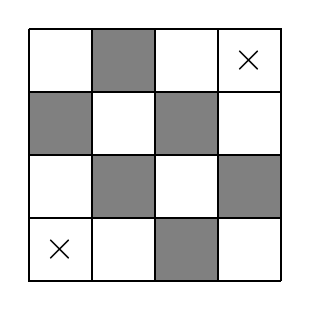
\begin{tikzpicture}[x=0.8cm,y=0.8cm,line width=0.7pt]
    \foreach \p in {(0,0),(2,0),(1,1),(3,1),(0,2),(2,2),(1,3),(3,3)}
        \fill[gray] \p rectangle ++(1,1);
    \draw[step=1] (0,0) grid (4,4);
    \fill[white] (0,0) rectangle (1,1); \draw (0,0) rectangle (1,1);
    \fill[white] (3,3) rectangle (4,4); \draw (3,3) rectangle (4,4);
    \node at (0.5,0.5){\Large \(\times\)};
    \node at (3.5,3.5){\Large \(\times\)};
\end{tikzpicture}}
\end{center}

Un domino placé sur l'échiquier recouvre toujours :

\begin{itemize}
    \item une case noire ;
    \item une case blanche.
\end{itemize}

Tout pavage par dominos doit donc recouvrir le même nombre de cases noires et
de cases blanches.

Un échiquier \(4\times4\) contient initialement \(8\) cases noires et
\(8\) cases blanches.

Les deux coins opposés retirés ont la même couleur. Il reste donc :

\[
6\text{ cases d'une couleur}
\qquad\text{et}\qquad
8\text{ cases de l'autre couleur}.
\]

Il est impossible que chaque domino recouvre une case de chaque couleur.

Ainsi,

\[
\boxed{
\text{L'échiquier mutilé ne peut pas être pavé par des dominos.}
}
\]

L'invariant est ici la différence entre le nombre de cases noires et le nombre
de cases blanches recouvertes.

\subsection{Sommes et sommes pondérées}

La somme totale des quantités présentes est parfois conservée.

Dans des problèmes plus délicats, la somme ordinaire varie, mais une
\textbf{somme pondérée} reste constante.

\paragraph{Exemple : trois boîtes.}

Trois boîtes \(A\), \(B\) et \(C\) contiennent respectivement \(a\), \(b\) et
\(c\) pierres.

Les opérations autorisées sont les suivantes :

\begin{itemize}
    \item transférer une pierre de \(A\) vers \(B\) ;
    \item retirer deux pierres de \(B\) et placer une pierre dans \(C\).
\end{itemize}

\begin{center}
\fitfig{%
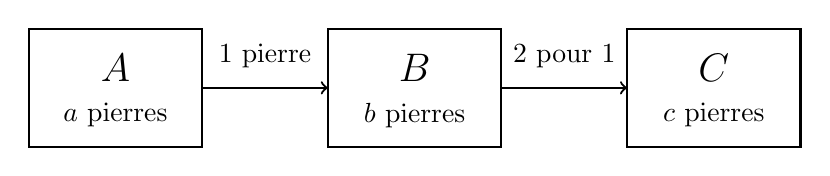
\begin{tikzpicture}[x=1cm,y=1cm,line width=0.8pt]
    \draw (0,0) rectangle (2.2,1.5);
    \draw (3.8,0) rectangle (6,1.5);
    \draw (7.6,0) rectangle (9.8,1.5);
    \node at (1.1,1){\Large \(A\)};
    \node at (1.1,0.4){\(a\) pierres};
    \node at (4.9,1){\Large \(B\)};
    \node at (4.9,0.4){\(b\) pierres};
    \node at (8.7,1){\Large \(C\)};
    \node at (8.7,0.4){\(c\) pierres};
    \draw[->] (2.2,0.75)--(3.8,0.75);
    \draw[->] (6,0.75)--(7.6,0.75);
    \node at (3,1.15){\(1\) pierre};
    \node at (6.8,1.15){\(2\) pour \(1\)};
\end{tikzpicture}}
\end{center}

La somme ordinaire \(a+b+c\) n'est pas conservée par la seconde opération.

Considérons plutôt

\[
I=a+b+2c.
\]

Lors de la première opération,

\[
(a,b,c)\longmapsto(a-1,b+1,c),
\]

donc

\[
I\longmapsto(a-1)+(b+1)+2c=I.
\]

Lors de la seconde opération,

\[
(a,b,c)\longmapsto(a,b-2,c+1),
\]

donc

\[
I\longmapsto a+(b-2)+2(c+1)=I.
\]

Ainsi,

\[
\boxed{I=a+b+2c}
\]

est un invariant.

À partir de l'état

\[
(8,0,0),
\]

on a

\[
I=8.
\]

L'état

\[
(0,1,3)
\]

a pour valeur

\[
I=0+1+2\times3=7.
\]

Il est donc inaccessible.

En revanche,

\[
(0,2,3)
\]

a la même valeur \(I=8\), et cet état est effectivement accessible.

\subsection{Le PGCD}

Le plus grand commun diviseur peut également rester constant.

On utilise l'identité fondamentale

\[
\boxed{
\gcd(a,b)=\gcd(a-b,b)=\gcd(a+b,b).
}
\]

\paragraph{Exemple.}

On part d'un couple d'entiers strictement positifs \((a,b)\). Une opération
permet de remplacer l'un des deux nombres par sa somme avec l'autre, ou, si
les deux nombres sont différents, par la différence positive des deux
(le plus grand moins le plus petit).

Le PGCD des deux nombres ne change jamais, car il est inchangé par l'identité
ci-dessus.

Ainsi, à partir de

\[
(18,30),
\]

tous les couples accessibles ont pour PGCD

\[
\gcd(18,30)=6.
\]

Comme \(\gcd(17,31)=1\neq 6\), il est impossible d'atteindre le couple

\[
(17,31),
\]

car

\[
\gcd(17,31)=1.
\]

\section{Monovariants}

Un invariant reste constant. Une autre idée très utile consiste à trouver une
quantité qui varie toujours dans le même sens.

\subsection{Définition}

Un \textbf{monovariant} est une quantité \(M\), calculée à partir de l'état,
qui :

\begin{itemize}
    \item augmente strictement après chaque opération ;
    \item ou diminue strictement après chaque opération,
\end{itemize}

\[
\boxed{
M(S')<M(S)
}
\]

ou

\[
\boxed{
M(S')>M(S).
}
\]

(\(S\) est un état et \(S'\) l'état obtenu après une opération.)

Si \(M\) est un \textbf{entier} qui diminue strictement et reste positif
(ou qui augmente strictement et reste majoré), il ne peut pas varier
indéfiniment : le processus s'arrête. Un monovariant permet notamment de
prouver :

\begin{itemize}
    \item qu'un processus doit s'arrêter ;
    \item qu'un état ne peut jamais réapparaître ;
    \item qu'un cycle est impossible.
\end{itemize}

\subsection{Exemple : l'algorithme des différences}

On considère deux entiers positifs \(a\) et \(b\).

Tant qu'ils sont différents, on remplace le plus grand par la différence des
deux nombres.

Par exemple,

\[
(18,30)
\longmapsto
(18,12)
\longmapsto
(6,12)
\longmapsto
(6,6).
\]

La somme

\[
M=a+b
\]

diminue strictement à chaque opération.

Elle reste pourtant un entier positif. Elle ne peut donc pas diminuer
indéfiniment.

Le processus doit s'arrêter.

Par ailleurs, le PGCD de \(a\) et \(b\) est invariant. Lorsque le processus
s'arrête, les deux nombres sont égaux. Leur valeur commune est donc le PGCD
initial.

Dans l'exemple,

\[
\gcd(18,30)=6.
\]

On obtient bien le couple final

\[
(6,6).
\]

Cet exemple utilise simultanément :

\[
\boxed{\text{un invariant : le PGCD}}
\]

et

\[
\boxed{\text{un monovariant : la somme \(a+b\)}}.
\]

\section{À retenir}

\small{
\begin{center}
\resizebox{\linewidth}{!}{%
\begin{tabular}{|c|c|c|}
\hline
\textbf{Outil} & \textbf{Comportement} & \textbf{Utilité principale} \\
\hline
Invariant & reste constant & prouver une impossibilité \\
\hline
Monovariant & augmente ou diminue & prouver la terminaison \\
\hline
Parité & reste modulo \(2\) & opérations modifiant un nombre pair d'objets \\
\hline
Congruence & reste modulo \(m\) & déplacements par multiples de \(m\) \\
\hline
Coloriage & classes de couleurs & pavages et déplacements \\
\hline
Somme pondérée & combinaison \(w_1x_1+\cdots+w_nx_n\) & compensations entre opérations \\
\hline
PGCD & diviseurs communs & opérations par sommes et différences \\
\hline
\end{tabular}%
}
\end{center}
}

\begin{center}
\fbox{
\begin{minipage}{0.9\linewidth}
\[
\boxed{
\text{Invariant différent}
\Longrightarrow
\text{état inaccessible}
}
\]

\[
\boxed{
\text{Entier qui diminue strictement et reste positif}
\Longrightarrow
\text{le processus finit par s'arrêter}
}
\]
\end{minipage}
}
\end{center}

\section{Exercices de compréhension}

\paragraph{Exercice 1.}
On dispose de \(20\) jetons, initialement tous blancs. À chaque opération, on
retourne exactement \(6\) jetons.

\begin{enumerate}
    \item Comment varie la parité du nombre de jetons noirs ?
    \item Peut-on obtenir exactement \(5\) jetons noirs ?
    \item Peut-on obtenir exactement \(8\) jetons noirs ? L'invariant suffit-il
    à conclure ?
\end{enumerate}

\paragraph{Exercice 2.}
Un entier est initialement égal à \(4\). À chaque opération, on peut lui ajouter
\(10\) ou lui retrancher \(15\).

\begin{enumerate}
    \item Quel reste modulo \(5\) est invariant ?
    \item Peut-on atteindre \(2026\) ?
    \item Peut-on atteindre \(2024\) ?
\end{enumerate}

\paragraph{Exercice 3.}
Un cavalier est placé sur une case noire d'un échiquier \(8\times8\). Un
déplacement du cavalier avance de deux cases dans une direction, puis d'une
case dans une direction perpendiculaire.

\begin{enumerate}
    \item Montrer qu'après chaque déplacement, il change de couleur de case.
    \item Peut-il revenir à sa case initiale après un nombre impair de
    déplacements ?
    \item Peut-il revenir à sa case initiale après un nombre pair de
    déplacements ? L'invariant suffit-il à répondre ?
\end{enumerate}

\paragraph{Exercice 4.}
Pour chacune des quantités suivantes, dire s'il s'agit plutôt d'un invariant ou
d'un monovariant :

\begin{enumerate}
    \item le PGCD dans l'algorithme des différences ;
    \item la somme des deux nombres dans ce même algorithme ;
    \item la parité du nombre de jetons noirs lorsqu'on retourne deux jetons ;
    \item le nombre de piles lorsqu'on fusionne deux piles de jetons en une seule.
\end{enumerate}

\section{Exercices faciles}

\paragraph{Exercice 5.}
Dix entiers sont initialement tous égaux à \(0\).

À chaque opération, on choisit exactement deux de ces entiers et on ajoute
\(1\) à chacun d'eux.

\begin{enumerate}
    \item Montrer que la parité du nombre d'entiers impairs est invariante.
    \item Peut-on obtenir une configuration contenant exactement un entier
    impair ?
    \item Peut-on obtenir une configuration contenant exactement deux entiers
    impairs ?
\end{enumerate}

\paragraph{Exercice 6.}
Un échiquier \(6\times6\) est privé de deux coins opposés.

\begin{enumerate}
    \item Combien contient-il initialement de cases noires et de cases blanches ?
    \item Les deux coins opposés ont-ils la même couleur ?
    \item Peut-on paver les cases restantes avec des dominos \(1\times2\) ?
\end{enumerate}

\paragraph{Exercice 7.}
On part du couple

\[
(84,30).
\]

À chaque opération, on peut remplacer l'un des nombres par la somme des deux
nombres, ou, s'ils sont différents, par leur différence positive (le plus grand
moins le plus petit).

\begin{enumerate}
    \item Montrer que le PGCD est invariant.
    \item Peut-on atteindre le couple \((15,21)\) ?
    \item Peut-on atteindre le couple \((12,18)\) ?
    \item Un couple d'entiers strictement positifs de PGCD \(6\) est-il
    toujours accessible ? (Indication : montrer que chaque opération peut être
    annulée par une opération autorisée.)
\end{enumerate}

\paragraph{Exercice 8.}
Des nombres entiers sont écrits aux sommets d'un triangle.

À chaque opération, on ajoute \(1\) aux nombres situés à deux sommets
différents.

\begin{enumerate}
    \item Montrer que la parité de la somme des trois nombres est invariante.
    \item En partant de \((0,0,0)\), peut-on atteindre \((1,1,1)\) ?
    \item Peut-on atteindre \((1,1,0)\) ?
\end{enumerate}

\section{Exercices \(+\)}

\paragraph{Exercice 9 --- Les trois boîtes.}
Trois boîtes \(A\), \(B\) et \(C\) contiennent respectivement \(a\), \(b\) et
\(c\) pierres.

Les opérations autorisées sont :

\begin{itemize}
    \item transférer une pierre de \(A\) vers \(B\) ;
    \item remplacer deux pierres de \(B\) par une pierre dans \(C\).
\end{itemize}

On part de la configuration

\[
(12,0,0).
\]

\begin{enumerate}
    \item Montrer que \(a+b+2c\) est invariant.
    \item Peut-on atteindre \((0,1,5)\) ?
    \item Peut-on atteindre \((0,2,5)\) ?
    \item Donner explicitement une suite d'opérations permettant d'atteindre
    \((0,2,5)\).
\end{enumerate}

\paragraph{Exercice 10 --- Pavage par carrés \(2\times2\).}
On considère un damier \(6\times6\).

On retire les quatre cases

\[
(1,1),\qquad(1,3),\qquad(3,1),\qquad(3,3),
\]

où \((i,j)\) désigne la case située sur la ligne \(i\) et la colonne \(j\)
(lignes et colonnes numérotées de \(1\) à \(6\)).

On souhaite paver les \(32\) cases restantes avec des carrés \(2\times2\).

\begin{enumerate}
    \item Colorier les cases avec quatre couleurs selon les parités de \(i\) et
    de \(j\).
    \item Montrer que tout carré \(2\times2\) recouvre exactement une case de
    chaque couleur.
    \item Vérifier que les quatre cases retirées ont la même couleur.
    \item En déduire que le pavage est impossible.
\end{enumerate}

\paragraph{Exercice 11 --- Pierres disposées en cercle.}
On dispose \(2n\) tas de pierres sur un cercle (\(n\geq2\)), numérotés
dans l'ordre : le tas \(2n\) est voisin du tas \(1\). Leurs tailles sont

\[
a_1,a_2,\dots,a_{2n}.
\]

À chaque opération, on choisit deux tas voisins et on ajoute une pierre à
chacun d'eux.

\begin{enumerate}
    \item Montrer que la somme alternée
    \[
    S=a_1-a_2+a_3-a_4+\cdots+a_{2n-1}-a_{2n}
    \]
    est invariante.

    \item On part de
    \[
    (1,0,0,\dots,0).
    \]
    Peut-on obtenir une configuration dans laquelle tous les tas ont la même
    taille ?

    \item Même question si l'on part de
    \[
    (1,1,0,\dots,0).
    \]
    L'invariant suffit-il à conclure ?
\end{enumerate}

\paragraph{Exercice 12 --- Produit invariant.}
Au moins quatre nombres non nuls sont écrits au tableau.

Une opération consiste à changer simultanément le signe de deux nombres.

\begin{enumerate}
    \item Montrer que le produit de tous les nombres est invariant.
    \item En partant de nombres tous positifs, peut-on obtenir exactement un
    nombre négatif ?
    \item Peut-on obtenir exactement quatre nombres négatifs ?
\end{enumerate}

\section{Exercices \(++\)}

\paragraph{Exercice 13 --- Jetons alignés.}
On considère \(n\) jetons alignés, initialement tous blancs.

À chaque opération, on retourne deux jetons voisins.

\begin{enumerate}
    \item Montrer que toute configuration accessible contient un nombre pair
    de jetons noirs.

    \item Soient \(i<j\). Montrer qu'en retournant successivement les paires
    \[
    (i,i+1),(i+1,i+2),\dots,(j-1,j),
    \]
    seuls les jetons situés aux positions \(i\) et \(j\) changent finalement
    de couleur.

    \item En déduire que toute configuration contenant un nombre pair de
    jetons noirs est accessible.

    \item Conclure qu'une configuration est accessible si et seulement si elle
    contient un nombre pair de jetons noirs.
\end{enumerate}

\paragraph{Exercice 14 --- Les quatre coins d'un rectangle.}
Une grille rectangulaire comporte \(m\geq2\) lignes et \(n\geq2\) colonnes. Toutes les
cases sont initialement blanches.

Une opération consiste à choisir deux lignes et deux colonnes, puis à changer
la couleur des quatre cases situées à leurs intersections.

\begin{enumerate}
    \item Montrer que, dans chaque ligne, la parité du nombre de cases noires
    est invariante.

    \item Montrer de même que, dans chaque colonne, cette parité est invariante.

    \item En déduire que toute configuration accessible possède un nombre pair
    de cases noires dans chaque ligne et dans chaque colonne.

    \item Réciproquement, considérer une configuration possédant cette
    propriété. Pour chaque case noire \((i,j)\) de cette configuration, avec
    \(i<m\) et \(j<n\),
    effectuer l'opération sur les lignes \(i,m\) et les colonnes \(j,n\).

    \item Montrer que cette procédure permet d'effacer toutes les cases noires.

    \item Conclure qu'une configuration est accessible si et seulement si
    chaque ligne et chaque colonne contient un nombre pair de cases noires
    (remarquer que répéter une même opération l'annule).
\end{enumerate}

\paragraph{Exercice 15 --- Invariant et monovariant.}
On considère une liste finie d'entiers positifs.

À chaque opération, on choisit deux nombres distincts \(a>b\) et on remplace
\(a\) par \(a-b\).

\begin{enumerate}
    \item Montrer que le PGCD de tous les nombres de la liste est invariant.
    \item Montrer que la somme de tous les nombres diminue strictement.
    \item En déduire que le processus doit s'arrêter.
    \item Décrire les configurations dans lesquelles aucune opération n'est
    possible.
    \item Que peut-on déduire sur la valeur finale commune des nombres ?
\end{enumerate}

\section{Problèmes complexes}

\paragraph{Problème 1 --- Le taquin de quinze pièces.}
Un taquin est constitué de \(15\) pièces numérotées et d'une case vide,
disposées dans une grille \(4\times4\).

Une opération consiste à déplacer dans la case vide une pièce voisine
horizontalement ou verticalement.

On part de la configuration ordonnée

\[
\begin{matrix}
1&2&3&4\\
5&6&7&8\\
9&10&11&12\\
13&14&15&\square
\end{matrix}
\]

Peut-on atteindre la configuration

\[
\begin{matrix}
1&2&3&4\\
5&6&7&8\\
9&10&11&12\\
13&15&14&\square
\end{matrix}?
\]

\emph{Indications :}

\begin{itemize}
    \item chaque déplacement échange la case vide et une pièce ;
    \item colorier la grille comme un échiquier ;
    \item si la case vide revient à sa position initiale, le nombre de
    déplacements est pair ;
    \item comparer la parité de la permutation des \(16\) objets.
\end{itemize}

\paragraph{Problème 2 --- Une opération algébrique.}
Les nombres

\[
x_1,x_2,\dots,x_n
\]

sont écrits au tableau.

À chaque opération, on choisit deux nombres \(x\) et \(y\), on les efface et
on écrit à leur place le nombre

\[
x+y-xy.
\]

Après \(n-1\) opérations, il ne reste qu'un seul nombre.

\begin{enumerate}
    \item Montrer que
    \[
    1-(x+y-xy)=(1-x)(1-y).
    \]

    \item Trouver une quantité multiplicative qui reste invariante au cours du
    processus.

    \item Montrer que le dernier nombre ne dépend pas de l'ordre des opérations.

    \item Exprimer ce dernier nombre en fonction de
    \(x_1,x_2,\dots,x_n\).

    \item Calculer le nombre final lorsque les nombres initiaux sont
    \[
    \frac12,\frac13,\frac14,\dots,\frac1{n+1}.
    \]
\end{enumerate}

\paragraph{Problème 3 --- Pavage par barres de longueur \(3\).}
On considère un damier \(10\times10\), dont on retire la case située sur la
première ligne et la deuxième colonne (lignes et colonnes numérotées de
\(1\) à \(10\), la case \((i,j)\) étant sur la ligne \(i\) et la colonne \(j\)).

Peut-on paver les \(99\) cases restantes à l'aide de rectangles \(1\times3\),
placés horizontalement ou verticalement ?

\emph{Indications :}

\begin{itemize}
    \item attribuer à la case \((i,j)\) la couleur déterminée par
    \[
    i+j\pmod 3;
    \]
    \item montrer que toute barre \(1\times3\) recouvre une case de chacune des
    trois couleurs ;
    \item compter le nombre de cases de chaque couleur avant et après le
    retrait.
\end{itemize}

\paragraph{Problème 4 --- Égalisation sur un cycle pair.}
Des entiers sont placés aux sommets d'un polygone à \(2n\) sommets
(\(n\geq2\)).

Une opération permet d'ajouter \(1\), ou de retrancher \(1\), aux nombres
situés à deux sommets voisins.

\begin{enumerate}
    \item Montrer que la somme alternée des nombres est invariante.
    \item Montrer que si tous les nombres peuvent être rendus égaux, alors la
    somme alternée initiale est nulle.
    \item Prouver réciproquement que, si la somme alternée initiale est nulle,
    alors il est possible de rendre tous les nombres égaux.
\end{enumerate}

\emph{Indication :} procéder successivement autour du polygone en corrigeant
les sommets les uns après les autres.

\paragraph{Problème 5 --- Une suite de transformations.}
On place les nombres

\[
1,2,3,\dots,2026
\]

au tableau.

À chaque opération, on choisit deux nombres \(a\) et \(b\), on les efface et
on écrit leur somme \(a+b\).

\begin{enumerate}
    \item Quelle quantité reste invariante ?
    \item Quel sera nécessairement le dernier nombre inscrit ?
    \item Le résultat dépend-il de l'ordre des opérations ?
    \item Combien d'opérations sont nécessaires ?
    \item Identifier un monovariant simple.
\end{enumerate}

